%-----------------------------------------------------------------------------
%	 Diseño e Implementación
%-----------------------------------------------------------------------------

\lhead[\thepage]{Diseño e Implementación \thechapter. \rightmark}
\rhead[Diseño e Implementación \thechapter.1 \leftmark]{\thepage}

%	Capitulo 6: Diseño e Implementación
\chapter{Diseño e Implementación}
\markboth{Diseño e Implementación}{Diseño e Implementación}
En este capitulo se presenta a partir del problema planteado una solución basada en una aplicación web que es capaz de poder tomar los datos de dispositivos IoT entre sensores y actuadores con los que interactuar, a través de la integración de diversas herramientas de visualización y control, incluyendo la posibilidad tanto de presentar indicadores de datos en tiempo real, así como también interactuar con data histórica para su análisis.\\

Todas las tecnologías aquí presentadas son software y hardware libre por lo que pueden ser adaptadas rápidamente según los requerimientos funcionales del problema y cumplen con legislativa local para poder ser exploradas a fondo. 

%	Sección uno: Diseño de la solución
\section{Diseño de la solución}
\lhead[\thepage]{\thesection. Diseño de la solución}
El diseño propuesto para examinar la solución al problema planteado pasa por dos etapas:
\begin{itemize}
\item Prototipos de uno o más dispositivos IoT que sean capaces de generar información real de su entorno, explorando los métodos más adecuados para poder llevar a cabo la tarea de transmitir información, así como explorar las posibilidades de procesamiento de cada dispositivo.
\item Aplicación web que incluya la posibilidad de visualizar los datos, monitorear y controlar los dispositivos IoT que se encuentren registrados. Para ello se integraran una serie de herramientas de software que aprovechen las mejores características de su diseño para poder cumplir con los objetivos planteados.
\end{itemize}

A continuación se presentan de manera detallada el diseño de ambos elementos:

\subsection{Prototipos de Dispositivos IoT}
Para los prototipos de los dispositivos IoT se contó con cuatro placas programables de distinta índole:
\begin{itemize}
\item Dos Raspberry Pi modelos 3 B.
\item Un Raspberry Pi Zero.
\item Un Arduino Uno R3.
\end{itemize}

Por el lado de los sensores y actuadores a integrar a esos dispositivos se ha contado con los siguientes elementos:
\begin{itemize}
\item Dos sensores de movimiento PIR HC-SR501.
\item Un sensor de test de nivel de agua Robodo Sen18.
\item Un sensor de temperatura DS1820.
\item Dos leds RGB.
\item Una fotorresistencia (LDR).
\item Un sensor de temperatura y humedad DHT11.
\item Dos leds color verde.
\item Dos leds color rojo.
\item Seis leds color blanco.
\item Un sensor de intensidad lumínica TSL2561.
\item Un buzzer HW-508.
\item Una pantalla LCD 16x2 I2C Hd44780.
\item Un Lector de tarjetas RFID RC522.
\item Un llavero RFID 100.
\item Una tarjeta RFID programable. 
\item Una cámara RaspiCam V1.  
\end{itemize}

Dado que los dispositivos Raspberry Pi pueden usar un sistema operativo completo estos pueden operar de manera independiente a otros dispositivos, no siendo el caso del dispositivo Arduino Uno se complementa su integración haciendo uso de una computadora Apple iBook G4 para poder recibir y enviar la data de manera inalámbrica.\\

Siendo la idea examinar variables y comportamientos de dispositivos en un ambiente de un hogar inteligente junto con la variedad de placas programables, sensores y actuadores disponible se sugieren la creación de 4 prototipos de dispositivos IoT distintos:

\begin{itemize}
\item Un prototipo de dispositivo IoT usando Arduino Uno (junto al computador iBook G4) para representar un artefacto que se coloque en exteriores para obtener y representar variables ambientales y de recursos comunes en esas áreas. Para ello se destinan un sensor PIR HC-501, un sensor de test de nivel de agua Robodo Sen18, Un sensor de temperatura DS1820, un Led RGB para representar de manera visual la temperatura y una fotorresistencia LDR de 10K (véase figura: \ref{fig:arduino1}).
\begin{figure}[htb]
\centering
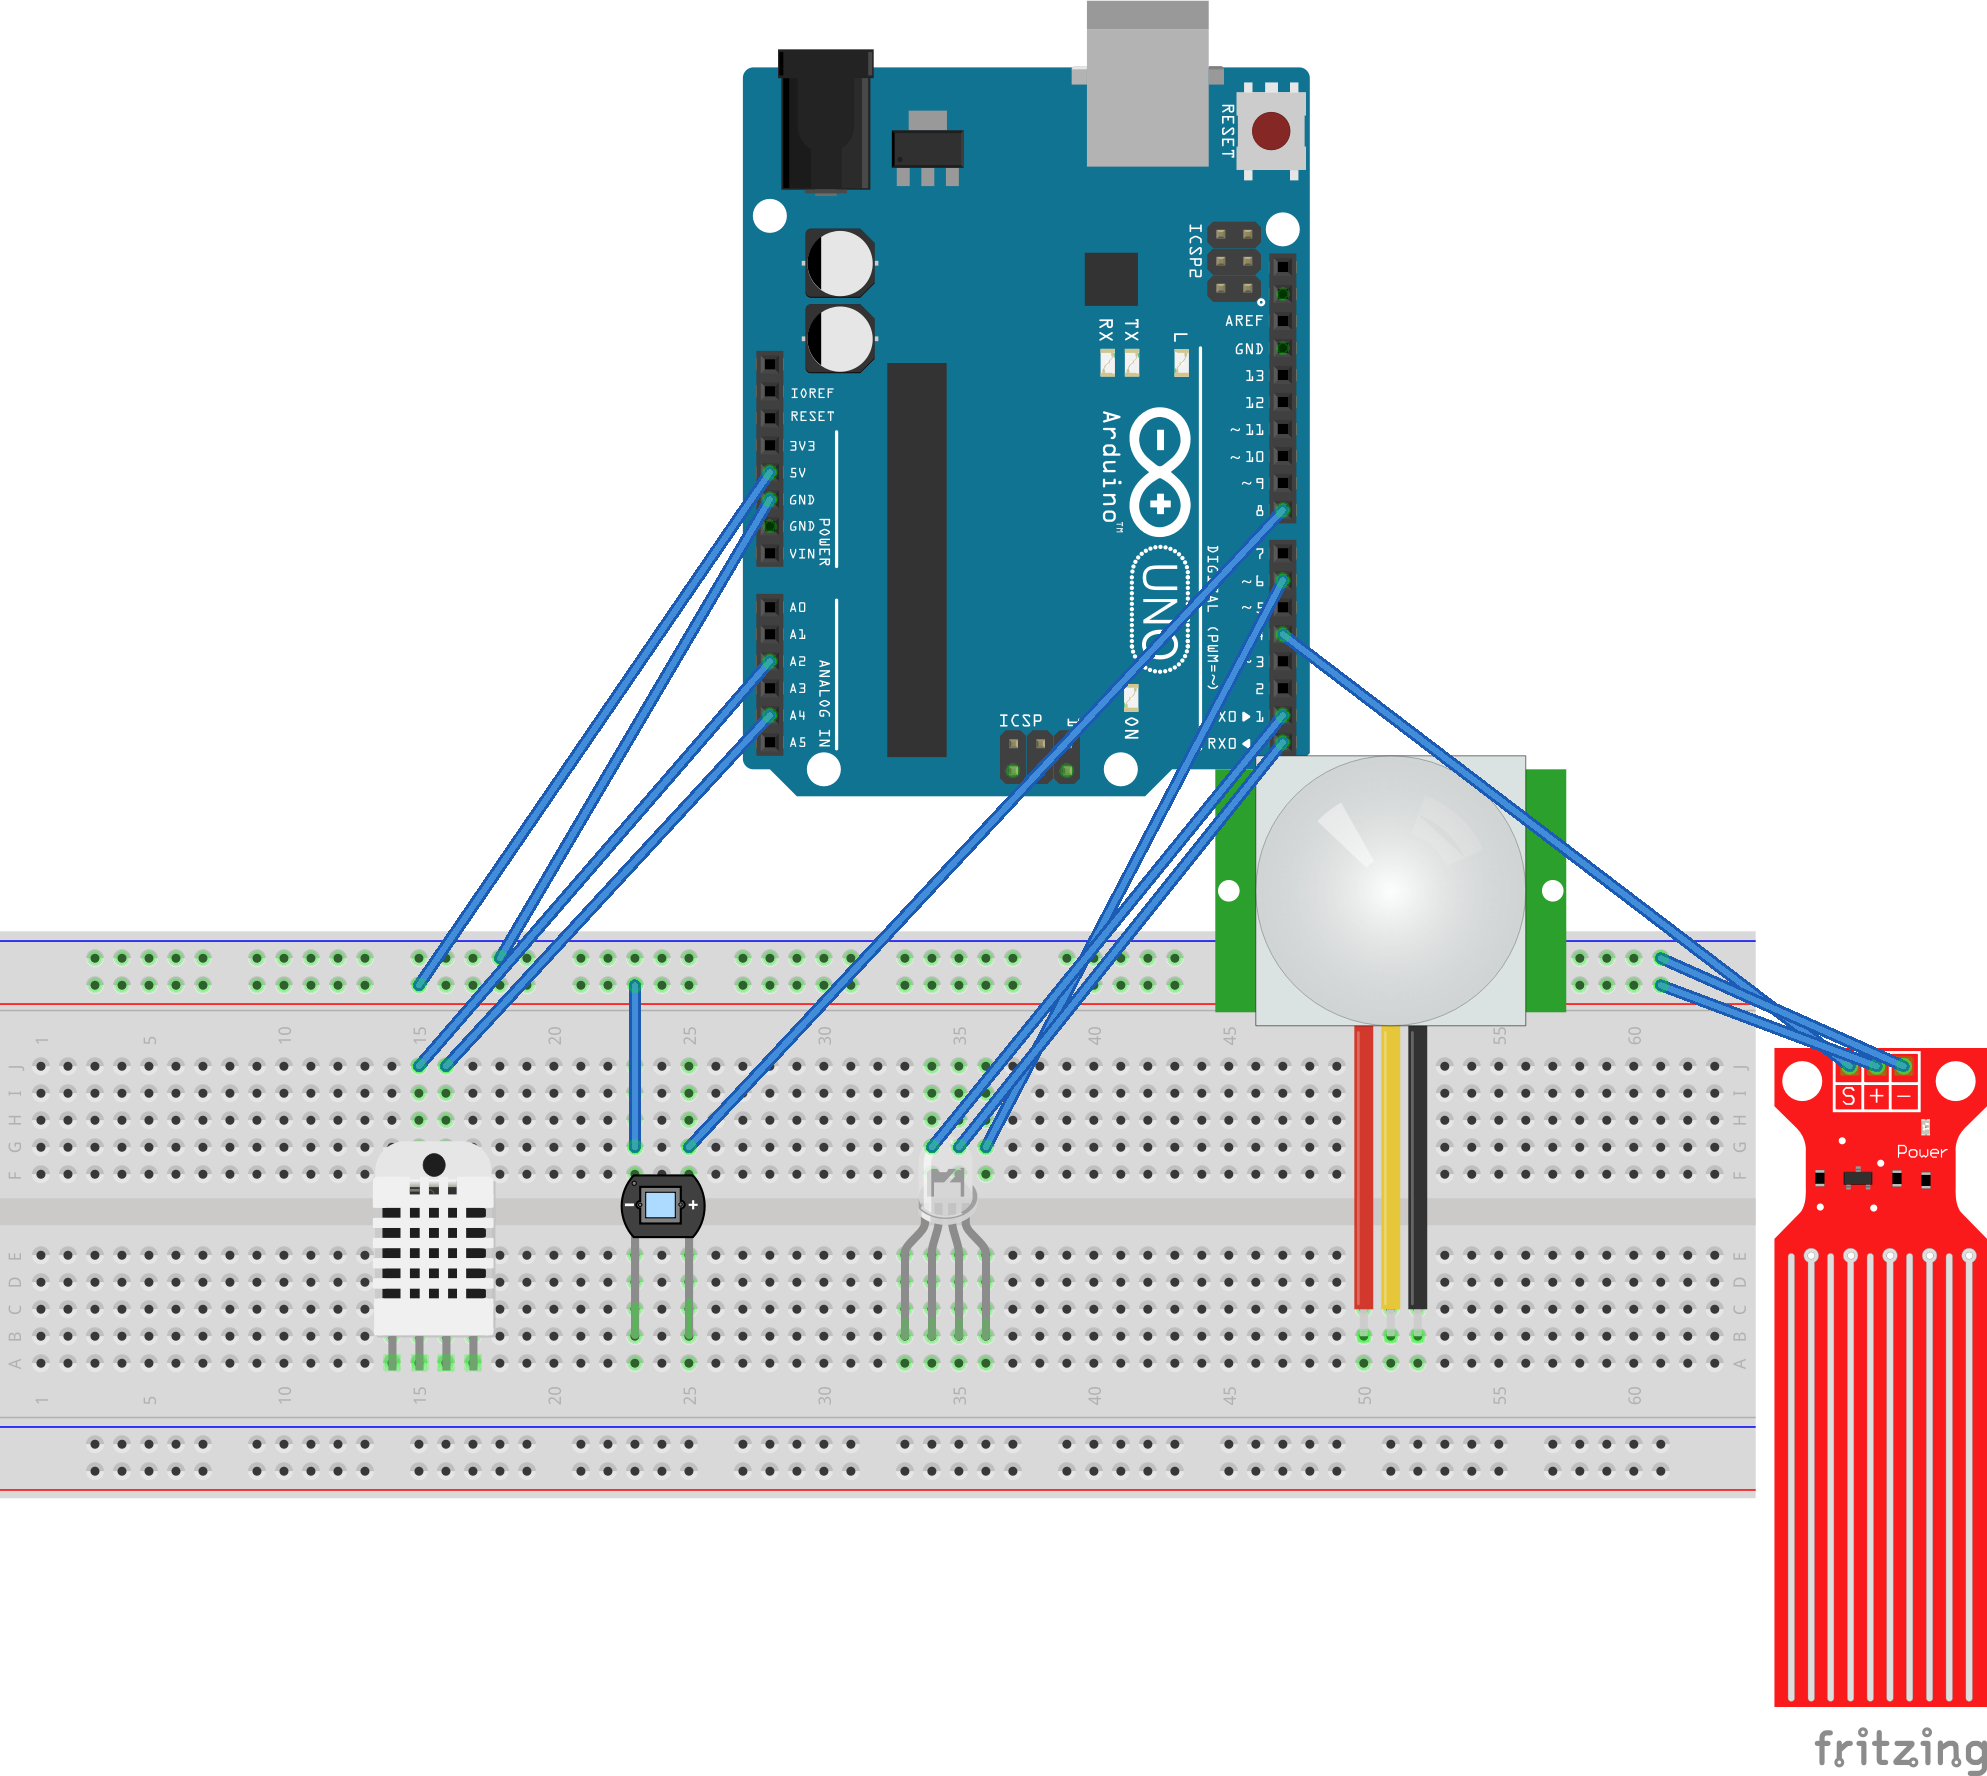
\includegraphics[scale=0.5]{./Figuras/arduino1.png}
\caption{Prototipo de dispositivo exterior usando Arduino Uno}
\label{fig:arduino1}
\vspace*{-10pt}
\end{figure}

\item Un prototipo de Dispositivo IoT usando un Raspberry Pi 3 Modelo B para representar un artefacto que se coloca en un espacio interior para obtener y representar variables ambientales y recursos comunes en el área. Para ello se harán uso de un sensor de temperatura y humedad DHT11, un Led RGB para representar de manera visual la temperatura, un sensor de medición de distancia usando ultrasonido HC-SR504, un led rojo y un led verde operacionales para indicar presencia de movimiento con el sensor de movimiento, un un buzzer y un servomotor que dada una cierta distancia con el sensor de movimiento se accionaran y a su vez tocara una melodía, un conjunto de 3 leds blancos para representar bombillos en una habitación y por último un sensor de intensidad lumínica TSL2561 para medir la intensidad de la luz en la habitación.(véase figura: \ref{fig:rpi3javier}).
\begin{figure}[htb]
\centering
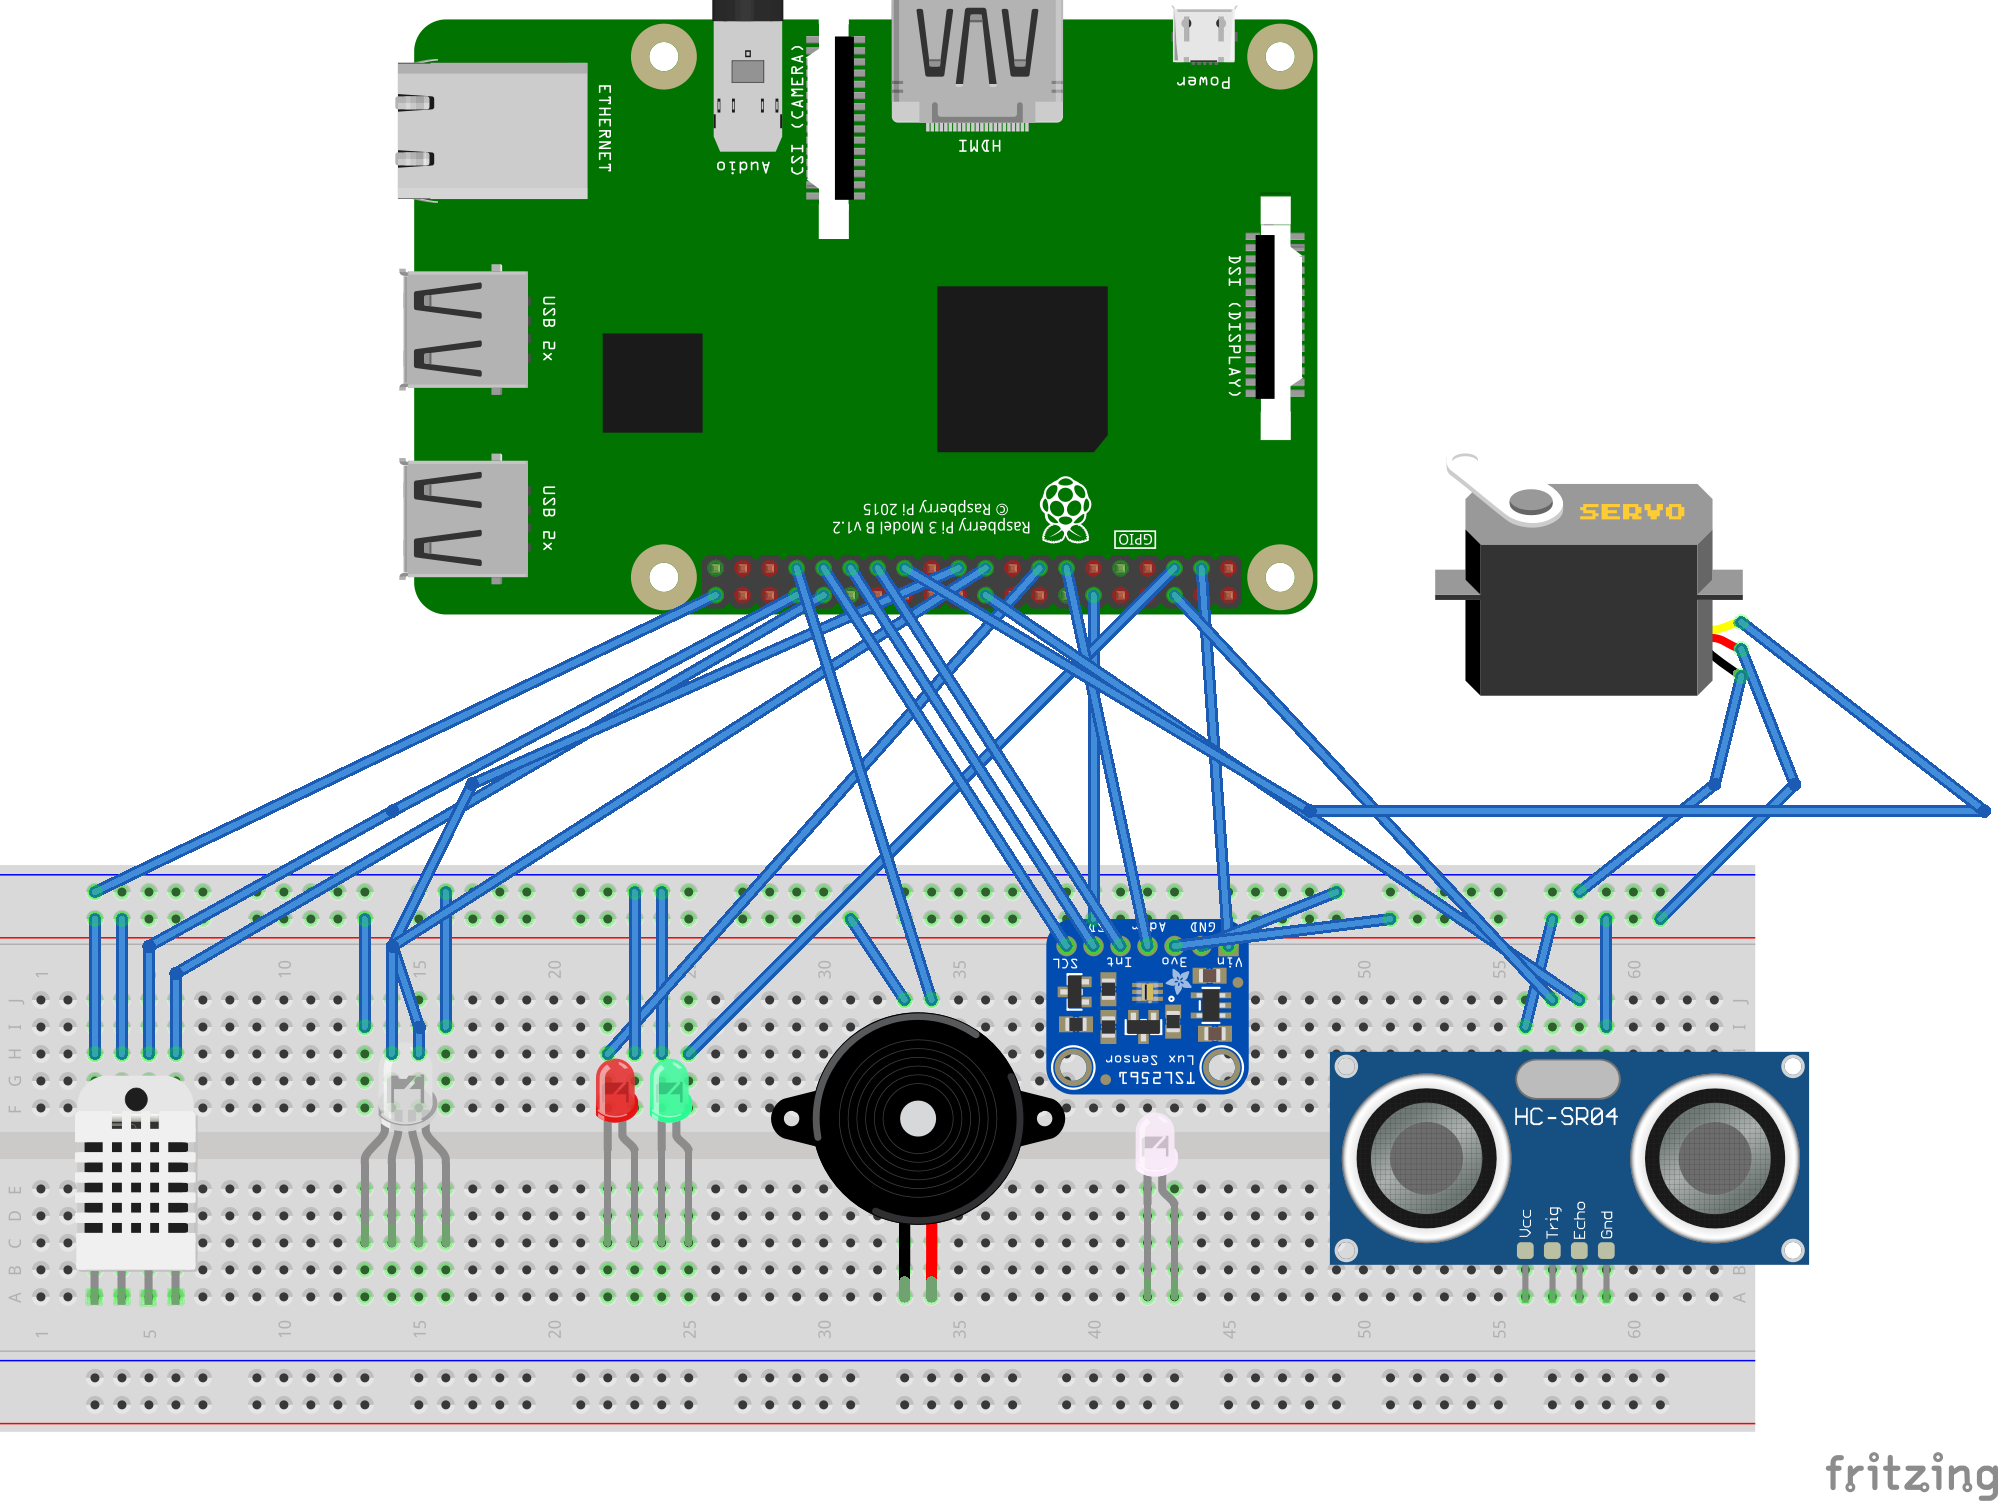
\includegraphics[scale=0.5]{./Figuras/rpi3javier.png}
\caption{Prototipo de dispositivo interior usando un Raspbery Pi 3 modelo B}
\label{fig:rpi3javier}
\vspace*{-10pt}
\end{figure}

\item Un prototipo de Dispositivo IoT usando un Raspberry Pi zero para representar un artefacto pensado para en variables de seguridad y acceso que se coloca en un espacio interior. Para ello se harán uso de un lector RFID RC522, una pantalla LCD para representar la hora y darle la bienvenida al usuario, un led rojo y un led verde operacionales para indicar existencia de movimiento gracias a un sensor PIR HC-SR501, 3 leds blancos para representar bombillos (que se activen con movimiento).(véase figura:\ref{fig:rpizero_diagram}).
\begin{figure}[htb]
\centering
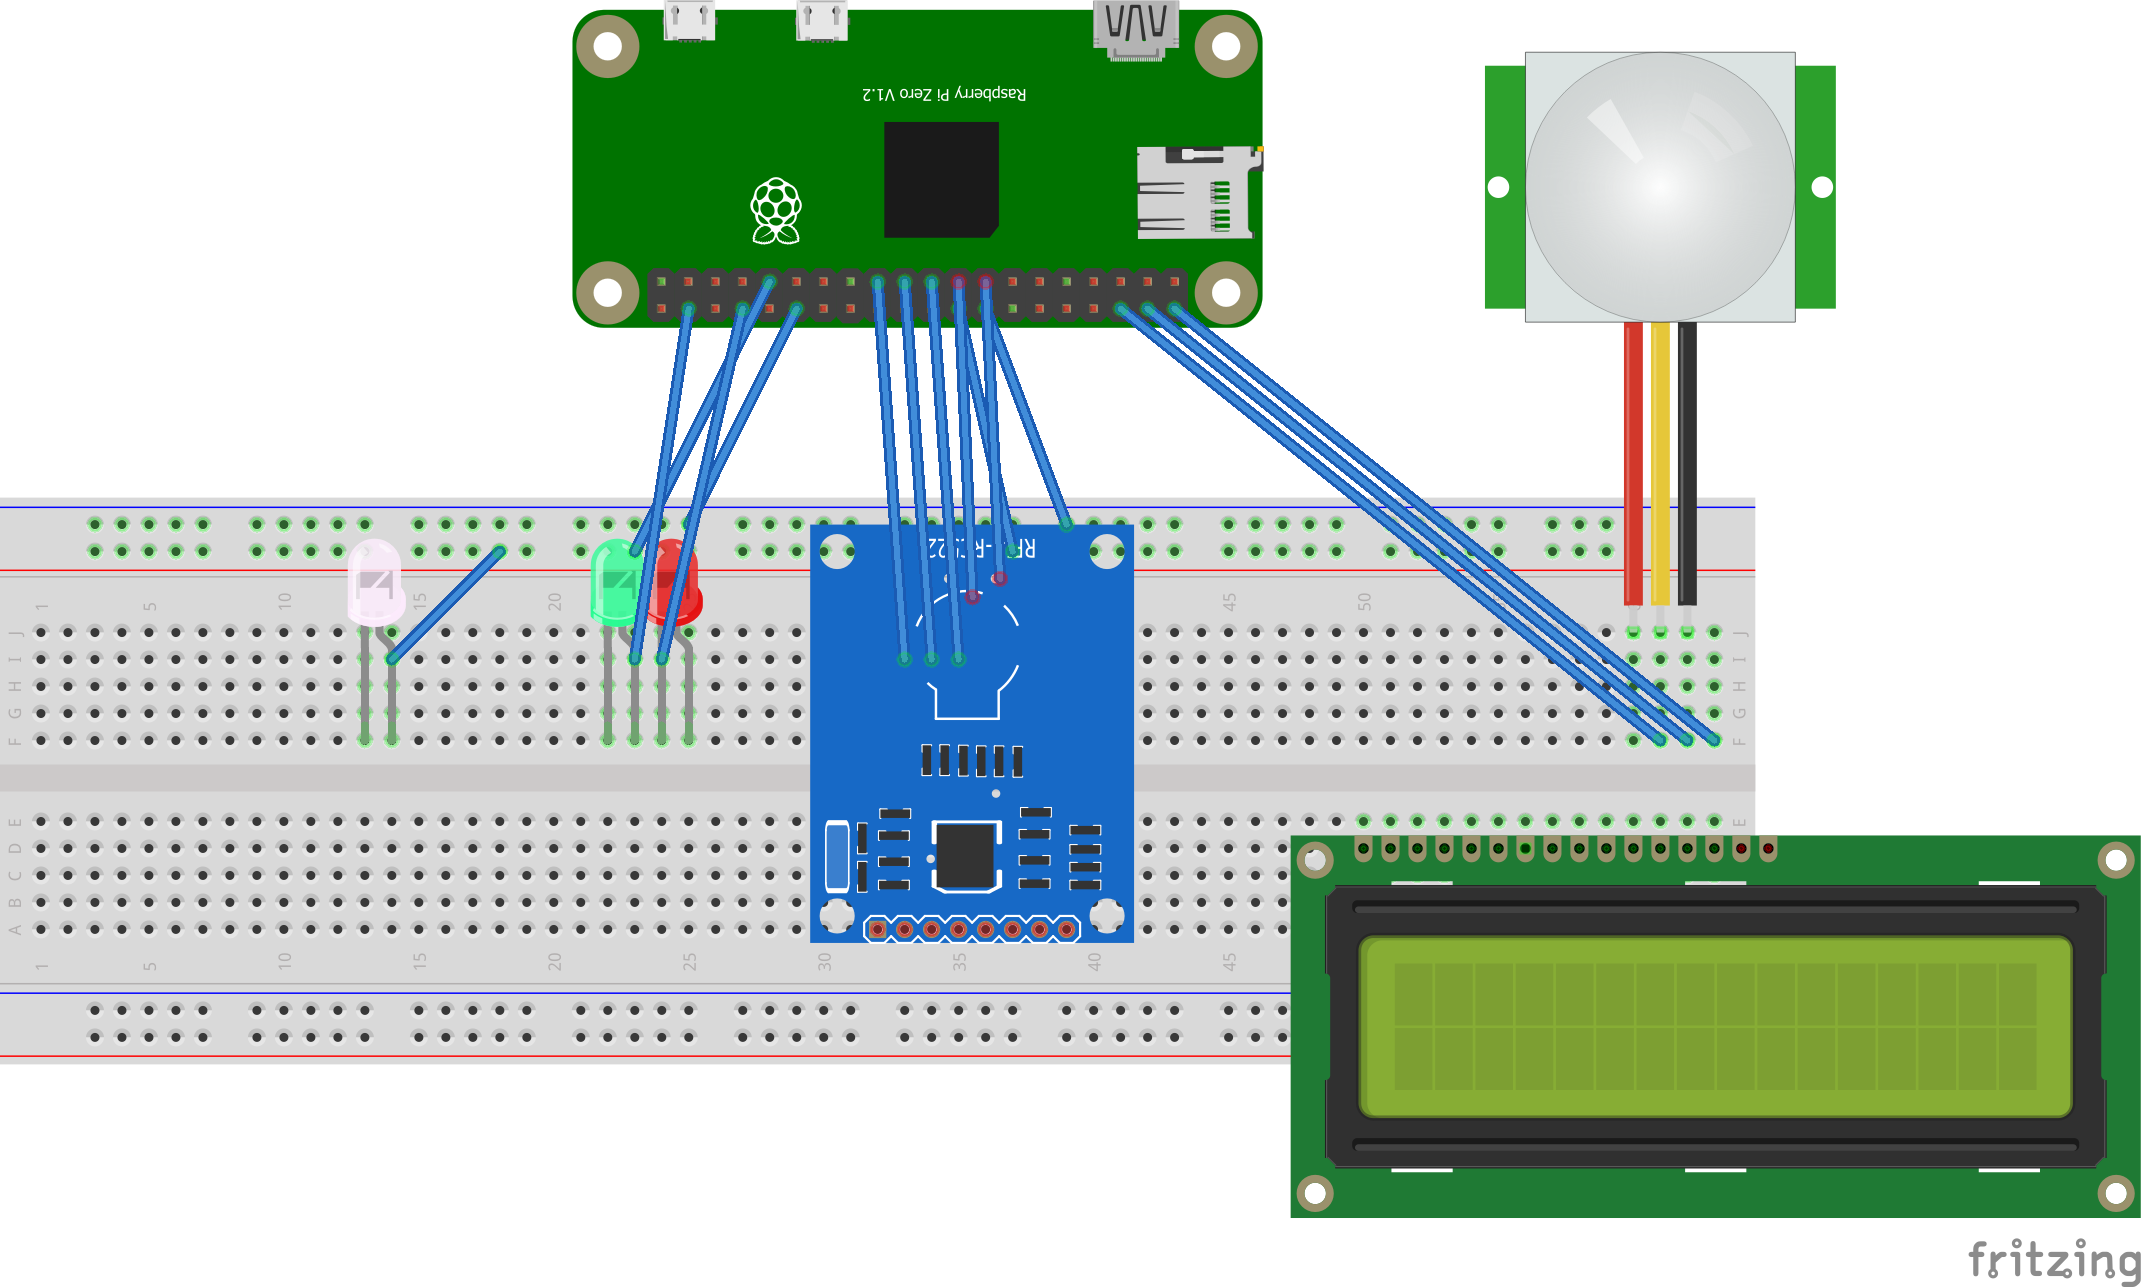
\includegraphics[scale=0.5]{./Figuras/rpizero_diagram.png}
\caption{Prototipo de dispositivo de seguridad usando un Raspbery Zero}
\label{fig:rpizero_diagram}
\vspace*{-10pt}
\end{figure}

\item Un prototipo de dispositivo IoT usando un Rapsberry Pi 3 Modelo B para representar una cámara inteligente capaz de detectar rostros de personas registradas y de desconocidos para alertar una posible intrusión usando un modelo de inteligencia artificial para ello. Se destina la cámara RaspiCam v1 para este particular.(véase figura:\ref{fig:rpipeter}). También dadas las capacidades computacionales de esta placa programable se establece que pueda usarse como punto de acceso para los otros prototipos y lugar de despliegue de la herramienta web HAMACA para visualización, monitoreo y control de los prototipos. 
\begin{figure}[htb]
\centering
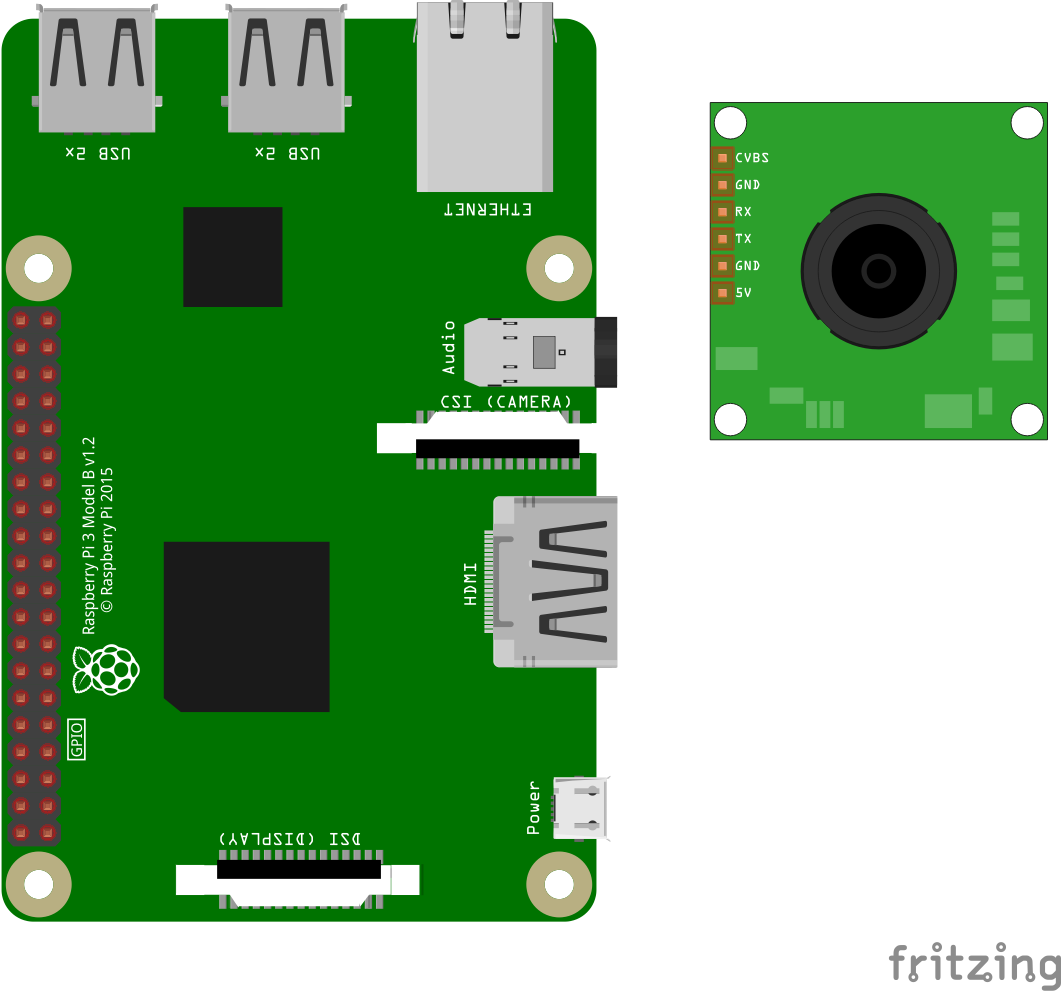
\includegraphics[scale=0.6]{./Figuras/rpipeter.png}
\caption{Prototipo de dispositivo de cámara de inteligente usando un Raspbery Pi 3 modelo B}
\label{fig:rpipeter}
\vspace*{-10pt}
\end{figure}

\end{itemize}

Con esta gama de distintos prototipos planteados para escenarios diferentes se hará obtención de data y generar acciones automáticas dependiendo del contexto que estos datos provean.  

\subsection{Software de Visualización, monitoreo y control HAMACA}
La parte mas importante del planteamiento del problema se traduce en la falta de soluciones que permitan visualizar datos históricos y en tiempo real, junto con la capacidad de monitorear el estado de los dispositivos y la posibilidad final de controlarlos y establecer rutinas mas allá de su programación inicial.\\

Para ello y examinando las diversas opciones de tecnologías estudiadas e investigadas durante el marco teórico del seminario se propone la creación de un software que funcione de la siguiente manera: 
\begin{itemize}
\item Una infraestructura básica que permita conectar a los dispositivos de manera centralizada, capaz de funcionar usando protocolos y estándares existentes, a la vez que este diseñado para su utilización en dispositivos IoT. Basados en la investigación previa por sus ventajas, robustez y simplicidad de uso se opta por utilizar el protocolo MQTT\cite{iotprotocols} bajo la implementación Mosquitto\cite{ALight2017}.

\item Dada la naturaleza no estructurada de los datos enviados por los dispositivos IoT, se requiere una base de datos que pueda almacenar fácilmente dichos valores. Se tiene que tener en cuenta que esta base de datos debería estar orientada a la utilización de datos históricos y en tiempo real (dimensión de tiempo). Es por ello que basados en la investigación previa realizada y teniendo en cuenta la naturaleza de los datos y las tareas que se esperan del sistema manejador de base de datos, se toma la decisión de usar InfluxDB\cite{influxdb}, que es una base de datos orientada a series de tiempo con alta integración con otras herramientas disponibles en el mercado.

\item  Una herramienta web que sea capaz de desplegar la información de sensores, actuadores tanto de manera histórica como en tiempo real, ademas de gestionar y centralizar el control de dispositivos y rutinas extras, con la posibilidad de tener acceso a ella basado en registro de usuarios y que estos sean capaces de crear cuadros de mando adaptados a las necesidades de sus dispositivos y requerimientos. Esta parte de la propuesta busca no crear todo una suite desde 0 sino aprovechar herramientas ya existentes para ello. Teniendo en cuenta eso, se decide en primer lugar crear una webapp usando el lenguaje de programación Python\cite{whatspython} en su version 3 con el framework Django\cite{django} bajo una base de datos Postgresql\cite{postgresql} para almacenamientos de los datos referentes a esta aplicación. En cuanto al tema de visualización y monitoreo se establece el uso integrado de la aplicación web Grafana\cite{grafana} y del mismo modo, para el control de dispositivos y de flujos de trabajos se acepta finalmente el uso de la herramienta web Node-Red\cite{nodered}

\end{itemize}

Con estos componentes definidos y después de discutir sobre la mejor manera de desplegar este conjunto de tecnologías, buscando facilidad de operación y manutención así como la portabilidad y la independencia de plataformas se decide utilizar la mayor cantidad de componentes posibles como contenedores. Para ello el uso de docker\cite{docker}, comenzando por las integraciones y otros componentes esenciales (figura \ref{fig:componentes_hamaca}).\\

\begin{figure}[htb]
\centering
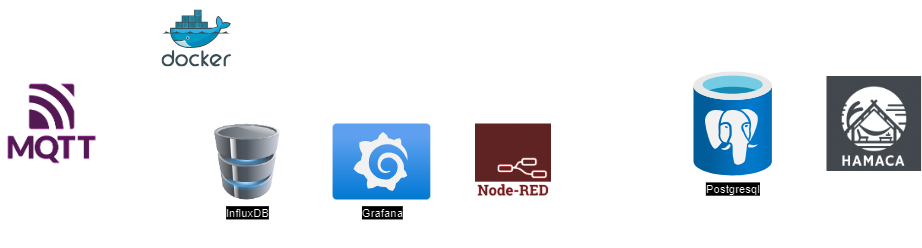
\includegraphics[scale=0.35]{./Figuras/componentes_hamaca.png}
\caption{Componentes sugeridos para la herramienta de visualización, monitoreo y control HAMACA}
\label{fig:componentes_hamaca}
\vspace*{-10pt}
\end{figure}

Finalmente con estos componentes se establecen las siguientes directrices:
\begin{itemize}

\item Se usara Mosquitto como Broker MQTT para las comunicaciones entre los dispositivos y aquel elemento que lleve la información a la base de datos. Este estará centralizado en el mismo dispositivo donde se alojará la aplicación web, aunque se recalca el hecho que pueden existir multiples brokers bajo la arquitectura de MQTT, así como también que el broker puede ser configurado de manera externa.


\item La webapp Hamaca seguirá el paradigma cliente-servidor, con un front-end marcado y distinto a su back-end. La aplicación web solo dependerá de la base de datos Postgresql para almacenar variables de configuración, estadísticas de uso (figura \ref{fig:psql_hamaca_db}) y aquellas que den soporte a la autenticación y gestión de usuarios (figura \ref{fig:django_schema})
\begin{figure}[!htb]
\centering
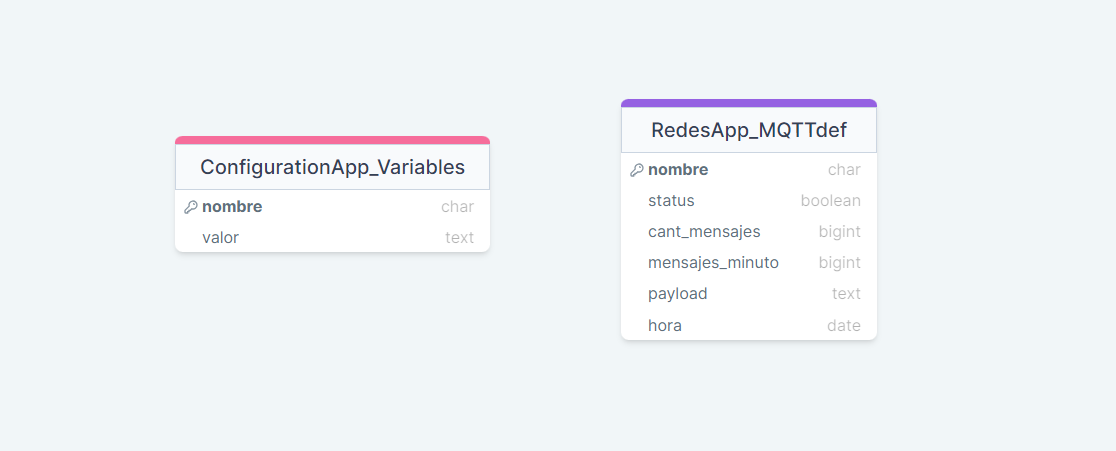
\includegraphics[scale=0.25]{./Figuras/psql_hamaca_db.png}
\caption{Modelo de la base de datos HAMACA}
\label{fig:psql_hamaca_db}
\vspace*{-10pt}
\end{figure}
\begin{figure}[!htb]
\centering
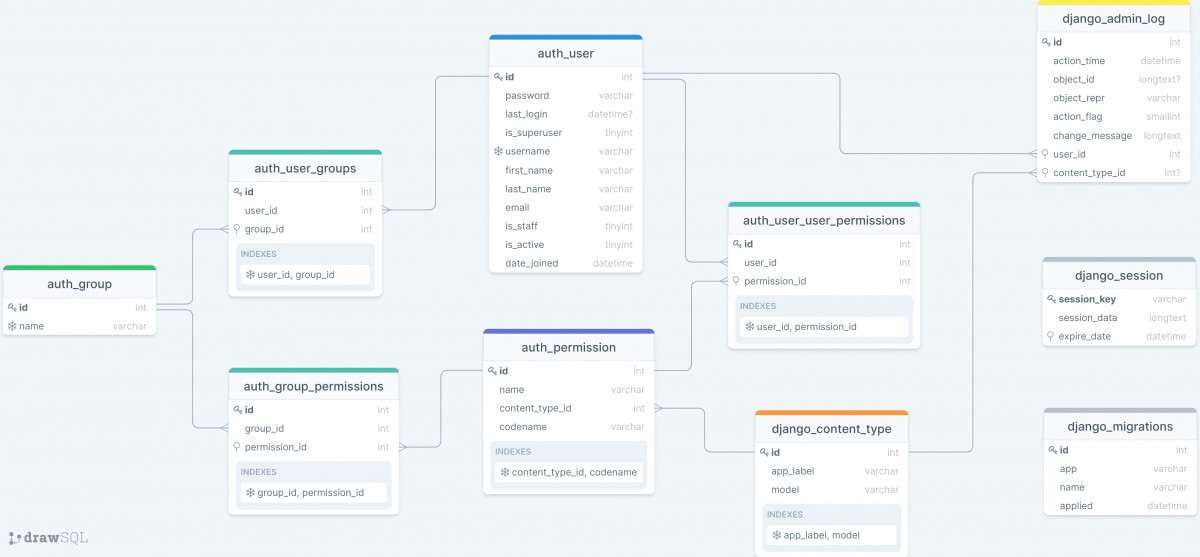
\includegraphics[scale=0.425]{./Figuras/django_schema.jpg}
\caption{Modelo autogenerado por el framework Django}
\label{fig:django_schema}
\vspace*{-10pt}
\end{figure}

\item La Base de datos Influxdb solo ha de ser consultada por la integración a Grafana para la visualización y monitoreo optimo de los datos haciendo uso de los dashboards configurables dentro de la aplicación. Grafana será embebido en la aplicación web HAMACA en su frontend. Al igual forma que la implementación de MQTT este puede existir en otro punto de red pero se sugiere el despliegue en el mismo dispositivo. 

\item La herramienta de control y de gestión de flujo de tareas automatizado Node-Red, al igual que Grafana será embebida sobre el frontend de la aplicación web HAMACA. Este componente podrá interactuar también con el broker MQTT para poder transmitir (y en algunos casos, también capturar directamente) los sensores y acturadores de los prototipos de dispositivos IoT.

\end{itemize}
De esta forma se presenta el diseño de la arquitectura de la solución para el problema de investigación como se puede notar en la figura \ref{fig:arquitectura_hamaca}
\begin{figure}[!htb]
\centering
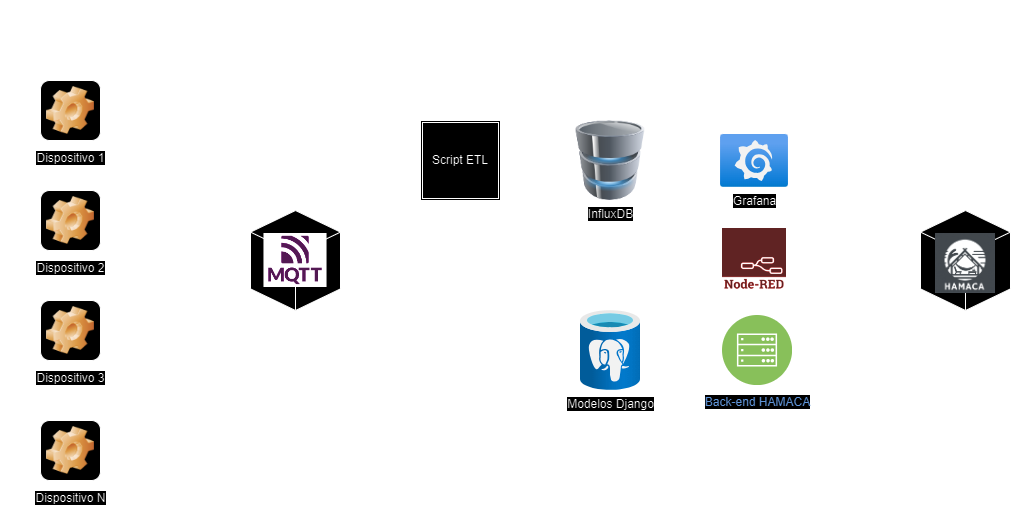
\includegraphics[scale=0.4]{./Figuras/arquitectura_hamaca.png}
\caption{Arquitectura de la solución propuesta}
\label{fig:arquitectura_hamaca}
\vspace*{-10pt}
\end{figure}

%	Sección dos: Implementación  de la solución 
\section{Implementación de la solución}
\lhead[\thepage]{\thesection. Diseño de la solución}


